\section*{Scope and reading protocol}
This edition combines a core narrative and the detailed English derivations
of all seventy-two source modules used or retained as supporting tools.
The historical source text is pinned to commit \texttt{99408ee}.
Stable R-identifiers are evidence locators. Both parts follow one logical
family order; the reader need not reconstruct a research chronology.

The manuscript presents a computer-assisted candidate argument for review.
Completeness of the English presentation does not establish mathematical
correctness, independent peer endorsement, or a complete formal proof.
Each quoted geometric implication must be checked on its actual domain;
each finite arithmetic exclusion must be checked against its supplied inputs.
The accompanying review ledger distinguishes completed editorial checks
from outstanding substantive proof-review obligations.

Appendix~\ref{app:M1} gives the sole normalization protocol: a local
target-relative cover-dominating replacement followed by complete
reclassification of any changed predicates. The optional stronger one-shot
global clamp is excluded. In particular, leaving one old leaf is not a
contradiction unless every resulting leaf is actually disposed of.

Global notation is fixed before the geometry begins. A technical lemma's
auxiliary symbols are scoped by its definitions. An explicit correspondence,
rather than a shared letter, governs a cross-module application. Tangent
and empty sections are different; the same original C/F must retain the
actual points used in every joint inequality.

The technical appendix also retains some supplementary historical routes.
Their presence does not assert that every such route is a necessary premise
of the final argument. For example, the R12 closure uses the early R11
membership reductions rather than its later optional angle-and-clamp route.
Module-level applicability notes and certificate references are part of
the material to be reviewed, not decorations.

\begin{figure}[htbp]\centering
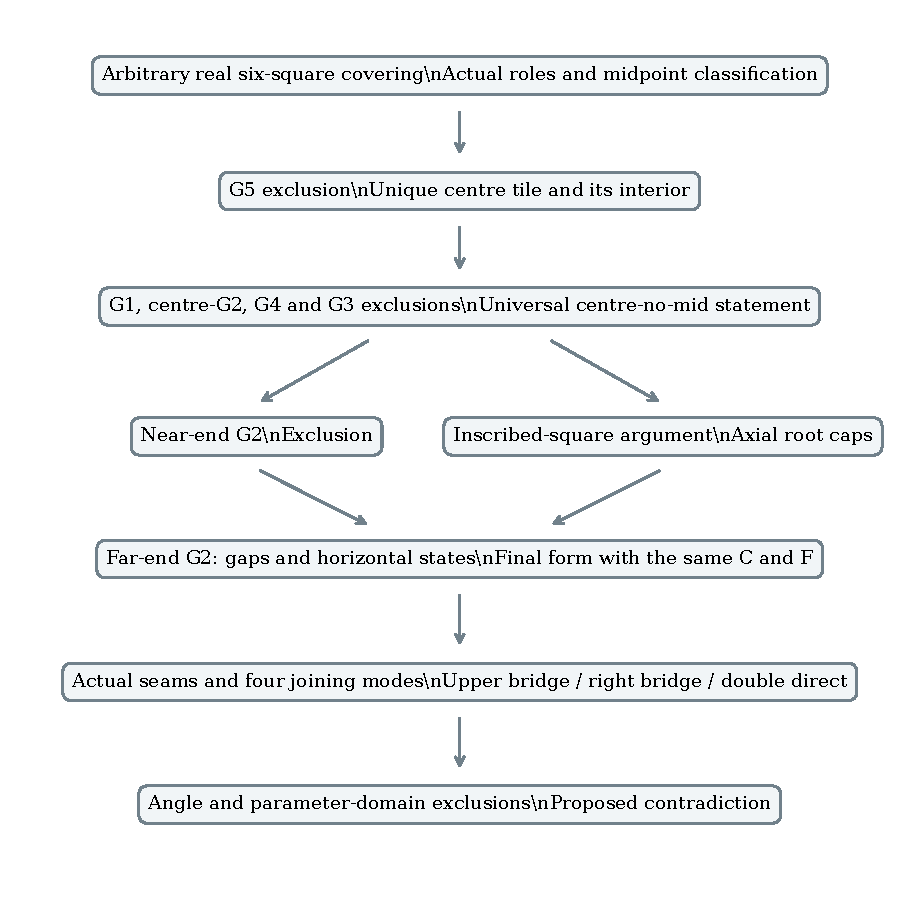
\includegraphics[width=.83\textwidth,height=.76\textheight,keepaspectratio]{figures/06_dependency_order.pdf}
\caption{Proposed dependency order. Each arrow is a geometric implication
requiring review; it is not an arithmetic verification result.}
\label{fig:route}\end{figure}
